\documentclass[tikz,border=3mm]{standalone}
\usepackage[siunitx]{circuitikz}
\usetikzlibrary{calc,positioning,arrows.meta}

\begin{document}

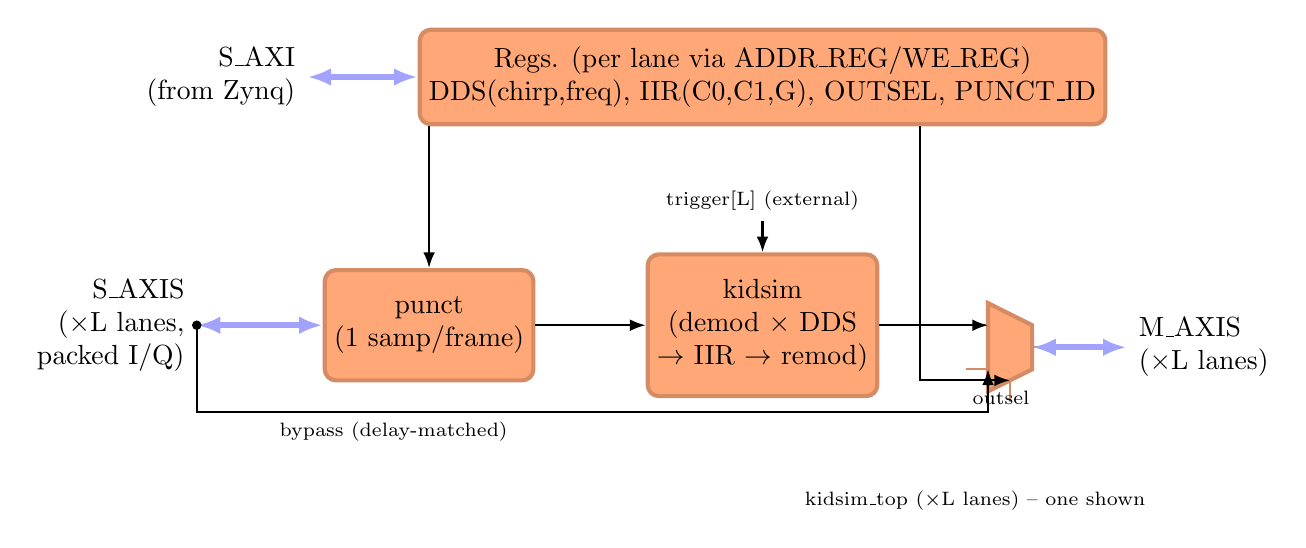
\begin{tikzpicture}
[box/.style={align=center, draw,rounded corners,minimum width=2cm,minimum height=1.2cm,draw={rgb,255:red,213; green,139; blue,99},fill={rgb,255:red,255; green,167; blue,118},line width=1.5pt},
outmux/.style={muxdemux, muxdemux def={Lh=2,NL=2,Rh=1,NR=1,NB=1,w=1},draw={rgb,255:red,213; green,139; blue,99},fill={rgb,255:red,255; green,167; blue,118},line width=0.75pt},
arrow/.style={line width=2.2pt,draw={rgb,255:red,162; green,163; blue,255},{Latex[length=3mm]}-{Latex[length=3mm]}},
single arrow/.style={line width=0.8pt,-{Latex[length=2mm]}},
node distance=0.5cm]

% Lane frame: one representative kidsim_top lane (x L total).
\node[box,minimum height=1.4cm] (punct) {punct\\(1 samp/frame)};

\node[box,right=1.4cm of punct,minimum height=1.8cm,minimum width=2.6cm] (kidsim) {kidsim\\(demod $\times$ DDS\\ $\to$ IIR $\to$ remod)};

\coordinate (temp) at ($(kidsim.east)+(1.1,0)$);
\node[outmux,anchor=lpin 1] (mux) at (temp) {};

% Bypass path (delay-matched raw input).
\coordinate (bypass start) at ($(punct.west)+(-0.4,-1.1)$);

% Regs.
\node[box,above=1.6cm of kidsim,minimum width=6.5cm] (regs) {Regs. (per lane via ADDR\_REG/WE\_REG)\\DDS(chirp,freq), IIR(C0,C1,G), OUTSEL, PUNCT\_ID};

% s_axis: packed input.
\draw[arrow] ($(punct.west)+(-1.6,0)$) coordinate (din) node[anchor=east,align=right] {S\_AXIS\\($\times$L lanes,\\ packed I/Q)} -- (punct.west);

% bypass tap + route.
\draw[fill] (din) circle (1.5pt);
\draw[single arrow] (din) |- (bypass start) -- (bypass start -| mux.blpin 2) -- (mux.blpin 2);
\node[font=\scriptsize] at ($(bypass start)+(1.3,-0.25)$) {bypass (delay-matched)};

% s_axi.
\draw[arrow] ($(regs.west)+(-1.4,0)$) node[anchor=east,align=right] {S\_AXI\\(from Zynq)} -- (regs.west);

% trigger.
\coordinate (temp) at ($(kidsim.north)+(0,0.4)$);
\draw[single arrow] (temp) node[anchor=south,font=\scriptsize] {trigger[L] (external)} -- (kidsim.north);

% Regs -> punct/kidsim/mux (config).
\draw[single arrow] (regs.south -| punct) -- (punct.north);
% outsel: tap well clear of kidsim's right edge (kidsim spans its own
% center +/-1.3) so this doesn't run down through the kidsim box itself.
\coordinate (outsel tap) at ($(regs.south)+(2.0,0)$);
\draw[single arrow] (outsel tap) -- (outsel tap |- mux.bbpin 1) -- (mux.bbpin 1) node[pos=0.9,below,font=\scriptsize] {outsel};

% punct -> kidsim.
\draw[single arrow] (punct.east) -- (kidsim.west);

% kidsim -> mux input 1 (processed).
\draw[single arrow] (kidsim.east) -- (mux.blpin 1);

% m_axis.
\draw[arrow] (mux.brpin 1) -- ++(1.2,0) node[anchor=west,align=left] {M\_AXIS\\($\times$L lanes)};

\node[font=\scriptsize,align=center] at ($(kidsim.south)+(2.7,-1.3)$) {kidsim\_top ($\times$L lanes) -- one shown};

\end{tikzpicture}

\end{document}
